\chapter{Implementacja}
\label{cha:implementacja}

Agent mając wiedzę na temat
\begin{itemize*}
\renewcommand{\labelitemi}{$\bullet$}
 \item akcji, które może wykonać,
 \item stanu, w jakim się znajduje,
 \item zasad, definiujących warunki otrzymania nagrody,
 \item polityki wybierania akcji
\end{itemize*}
jest w stanie dostosować swoje kolejne działania (wybrane akcje), tak aby uzyskać jak
najlepszy wynik w kolejnych iteracjach symulacji. Celem agenta jest dotarcie do punktu końcowego, zdobywając jak 
największą nagrodę. \\
\indent Po osiągnięciu celu symulacja jest resetowana, jej wynik jest zapisywany. Robot ucząc się na podstawie 
poprzednio dokonanych wyborów, buduje tablicę mapującą stan-akcja $Q(S, A)$ do konkretnej wyliczonej wartości. W 
programie do przedstawienia wartości tablicy stan-akcja $Q(S, A)$ wykorzystano wielowymiarową tablicę.

\section{Tablica stan-akcja $Q(S, A)$}

Tablica $Q(S, A)$ jest to struktura danych przechowująca wszystkie stany i możliwe do wykonania w nich akcje. Każdej z tych akcji przyporządkowana jest odpowiednia wartość, która jest poddawana modyfikacji przez odpowiedni algorytm uczenia ze wzmocnieniem.
Ostatecznym celem działania algorytmu jest uzyskanie takich informacji w strukturze $Q(S, A)$, aby robot korzystając z polityki optymalnej (tzn. takiej, w której agent wybiera zawsze najlepszą według niego akcję) wykonał cel z jak najlepszym wynikiem.

TODO PRZYKŁADOWA REPREZENTACJA

\section{Polityka wyboru akcji}
\label{sec:politykawyboru}

Agent mając do dyspozycji jedną z możliwych akcji $a$ ze zbiory wszystkich akcji $A$, musi podjąć decyzje, która akcję ma wybrać jako następną. W tej implementacji rozważane są dwie polityki
\begin{enumerate}
	\item $\epsilon$-greedy policy
	\item optimal policy
\end{enumerate}

\subsection{Równowaga pomiędzy eksploracją, a eksploatacją}
Od wyboru polityki zależy stopień eksploracji algorytmu. Gdyby agent za każdym razem wybierał najbardziej korzystną według niego akcję, byłby podatny na zakleszczenie w nieoptymalnym rozwiązaniu. Wprowadzając pewną losowość wyboru akcji agent, będzie w stanie odkryć nowe rozwiązania, nawet jeżeli według jego aktualnej wiedzy znalazł to najbardziej optymalne. Powstało dużo prac dokładniej badających to zagadnienie \ref{thrun1992efficient}, \ref{wiewiora2004efficient}.

\subsection{$\epsilon$-greedy policy}

Polityka $\epsilon$-greedy jest strategią wyboru akcji polegającą na wyborze losowej akcji z prawdopodobieństwem $\epsilon$, a w przeciwnym wypadku wybranie najbardziej korzystnej. Agent wybiera akcję, która według niego będzie najbardziej korzystna z prawdopodobieństwem $1-\epsilon$, a w przeciwnym wypadku wykonuje akcję losową. Parametr $\epsilon$ jest regulowany zależnie od potrzeb i musi spełniać zależność $0 < \epsilon < 1$.

\subsection{Optimal policy}

Polityka optymalna, agent za każdym razem wybiera najkorzystniejszą według jego wiedzy akcję.

\section{Symulacja graficzna}
\label{sec:symulacjagraficzna}

Jako symulację graficzna działania algorytmu wykorzystano figury geometryczne reprezentujące: agenta, przeszkody, 
granice i cel.
Agent porusza się na dwuwymiarowej przestrzeni o wymiarach $50*50$ pikseli.

Przykładowy stan środowiska w symulacji przedstawiono na rys. \ref{fig:symulacja}, \ref{fig:symulacja2}.

\begin{figure}[h!]
    \centering
    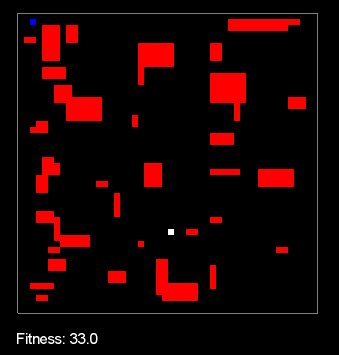
\includegraphics[scale=0.4]{symulacja}
    \caption{Przykładowy stan symulacji}
    \label{fig:symulacja}
\end{figure}

\begin{figure}[h!]
    \centering
    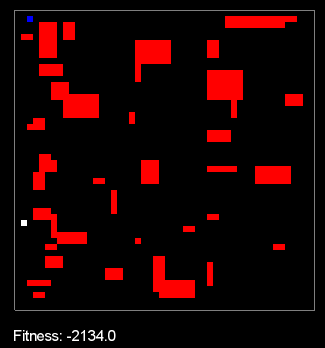
\includegraphics[scale=0.4]{symulacja2}
    \caption{Przykładowy stan symulacji}
    \label{fig:symulacja2}
\end{figure}

Na rys. \ref{fig:symulacja}, \ref{fig:symulacja2}, można zauważyć następującą reprezentacje obiektów jako kolor:
\begin{itemize}
\renewcommand{\labelitemi}{$\bullet$}
 \item czerwony - przeszkoda,
 \item biały - agent,
 \item niebieski - nagroda,
 \item szary - granica.
\end{itemize}


\section{Reprezentacja stanu}
\label{sec:reprezentacjastanu}

Stan w jakim znajduje się aktualnie robot jest przedstawiony w postaci siatki $3*3$. Agent jest świadomy obiektów 
znajdujących się nad nim, pod nim oraz po jego prawej i lewej stronie.
Agent może napotkać następujące obiekty
\begin{description}
%\renewcommand{\labelitemi}{$\bullet$}
 \item przeszkoda $(O)$, robot \textbf{może} wejść na przeszkodę, jednak traci za to określoną liczbę punktów;
 \item nagroda $(P)$, stan końcowy. Gdy agent osiąga cel symulacja zapisuje wynik działania i uruchamia się kolejny 
epizod nauki robota;
 \item granica $(B)$, granica jest obiektem wyznaczającym pole symulacji, dlatego też nie jest możliwe przemieszczenie 
się na nią;
  \item puste pole $(E)$, pole nie zawierające żadnego z pozostałych obiektów;
\end{description}
 
Przykładowe stany w jakich może się znaleźć robot przedstawiono na rys. \ref{fig:grid1}, \ref{fig:grid2}, 
\ref{fig:grid3} i \ref{fig:grid4}.

\begin{figure}[H]
    \centering
    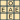
\includegraphics[scale=10]{grid1}
    \caption{Agent graniczy od górnej strony z przeszkodą, natomiast w pozostałych kierunkach znajdują się puste pola}
    \label{fig:grid1}
\end{figure}

\begin{figure}[H]
    \centering
    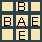
\includegraphics[scale=10]{grid2}
    \caption{Agent graniczy od góry i lewej strony z granicą, oznacza to, że robot znajduje się w górnym lewym rogu 
mapy, a jedynymi akcjami jakie może wykonać to ruch w prawo i ruch w dół}
    \label{fig:grid2}
\end{figure}

\begin{figure}[H]
    \centering
    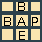
\includegraphics[scale=10]{grid3}
    \caption{Agent graniczy od góry i lewej strony z granicą, a od prawej z stanem końcowym. Agent wykonując 
ruch w prawo osiągnie swój cel, powodując tym samym zakończenie i zresetowanie symulacji}
    \label{fig:grid3}
\end{figure}

\begin{figure}[H]
    \centering
    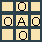
\includegraphics[scale=10]{grid4}
    \caption{Agent graniczy z każdej strony z przeszkodą, jakikolwiek ruch powoduje utratę punktów}
    \label{fig:grid4}
\end{figure}

\subsection{Akcje}
\label{subsec:akcje}

Robot znajdując się w dowolnym stanie nie graniczącym z obiektem $B$ (granicą), jest w stanie wykonać jedną z czterech 
akcji:

\begin{enumerate}
 \item ruch do góry,
 \item ruch do dołu,
 \item ruch w prawo,
 \item ruch w lewo.
\end{enumerate}

Agent \textbf{nie może} przemieścić się na granicę, w związku z czym w przypadku sąsiedztwa z granicą, robot posiada 
ograniczony zakres ruchów. 

\subsection{Wybór algorytmów}
\label{subsec:wyboralgorytmow}

Do implementacji inteligentnego zachowania agenta, wybrano algorytm Q-learning z dziedziny uczenia ze wzmocnieniem.



\subsubsection{Q-learning}
\label{subsubsec:qlearning}

Algorytm Q-learning \cite{watkins1992q} jest off-policy

\subsubsection{SARSA}
\label{subsubsec:sarsa}

\section{Wykorzystane technologie}
\label{sec:wykorzystanetechnologie}

Java 8 kod został napisany w języku Java. Do generowania grafiki została wykorzystana biblioteka LibGDX. W celu notowania wyników do plików kalkulacyjnych została wykorzystana biblioteka Apache POI.

\section{Napotkane problemy}
\label{sec:napotkaneproblemy}

Przy projektowaniu aplikacji, największy problem stanowiło odpowiednie przedstawienie aktualnego stanu środowiska i robota. Nieodpowiednie odwzorowanie stanu, może powodować niepoprawną naukę agenta.
Zakładając rozmiar mapy $50*50$, można zauważyć, że przy naiwnej reprezentacji stanu, tzn. takiej, w której każda możliwa kombinacja stanu mapy jest reprezentowana osobno, powstaje ogromna ilość możliwych akcji w tablicy wartości $Q(S,A)$ 
Ostatecznie postanowiono przedstawić stan w postaci siatki $3*3$.
Reprezentacja stanu
Testowanie działania algorytmów

\section{Wynik działania}
\label{sec:wynikdzialania}


%---------------------------------------------------------------------------














